\chapter{Implementation}\label{C:imp}


//TODO rename sections to reflect work done
\section{Mechanical Design}

\begin{itemize}
    \item Go into 3d printing/laser cutting refinement, testing and adjustment
    \item Tolerance and dimension adjustment
    \item Noted changed and drawback from design
\end{itemize}

\subsection{Rotating Pipette Mount}

\subsection{Z micrometer Control}
\begin{itemize}
    \item Note initially large vibrations as z decreases, caused be loose tolerance, too small coupler. Caused droplet to prematurely detach at larger values.
\end{itemize}


\begin{figure}[h]
    \centering
    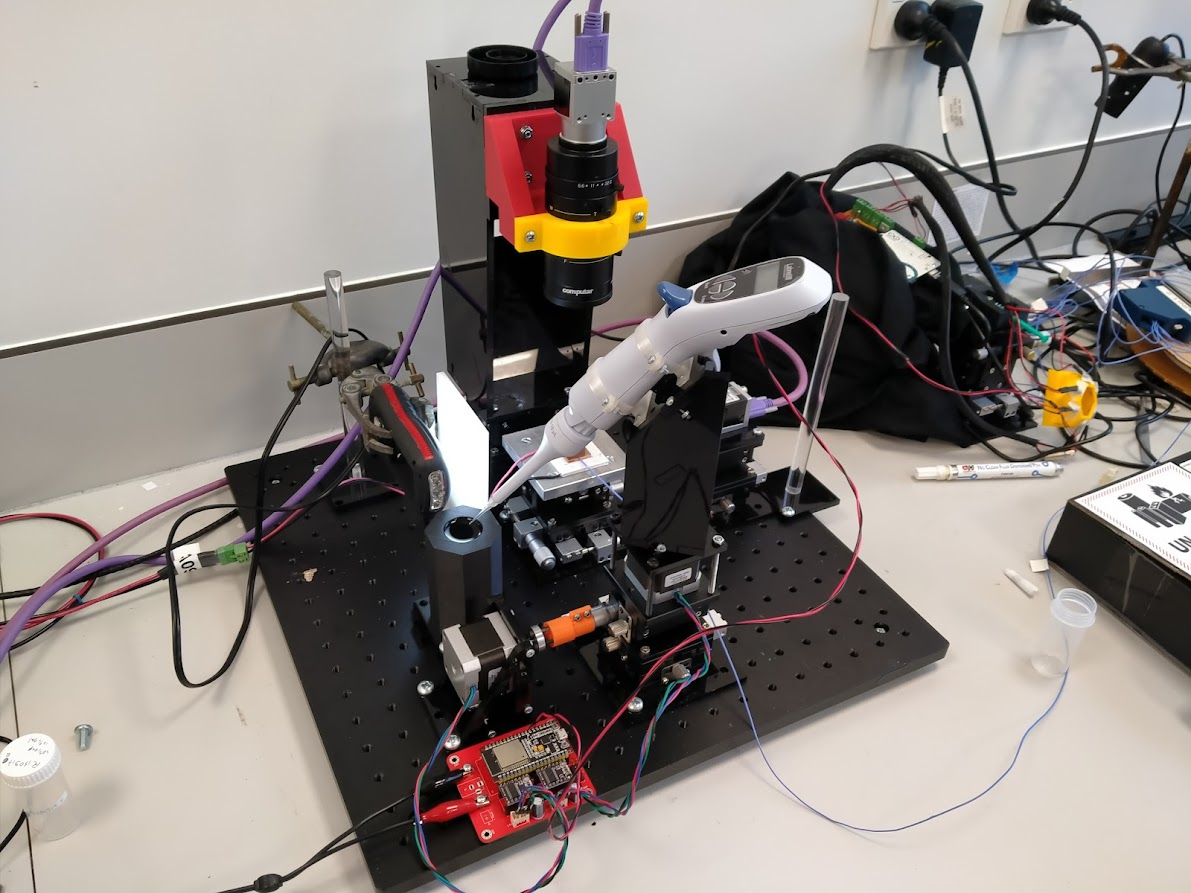
\includegraphics[width=0.4\textwidth]{img/full_sys.jpg}
    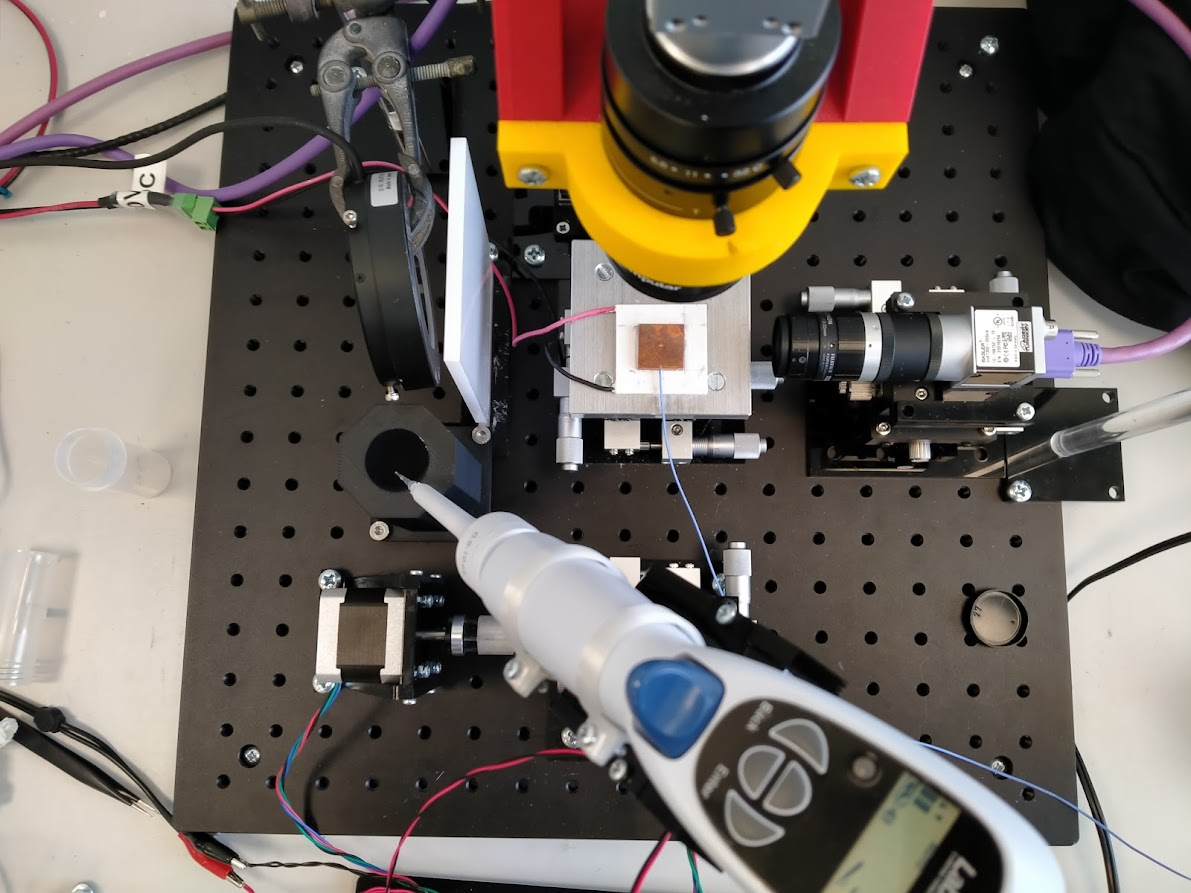
\includegraphics[width=0.4\textwidth]{img/impl_sys_top.jpg}
    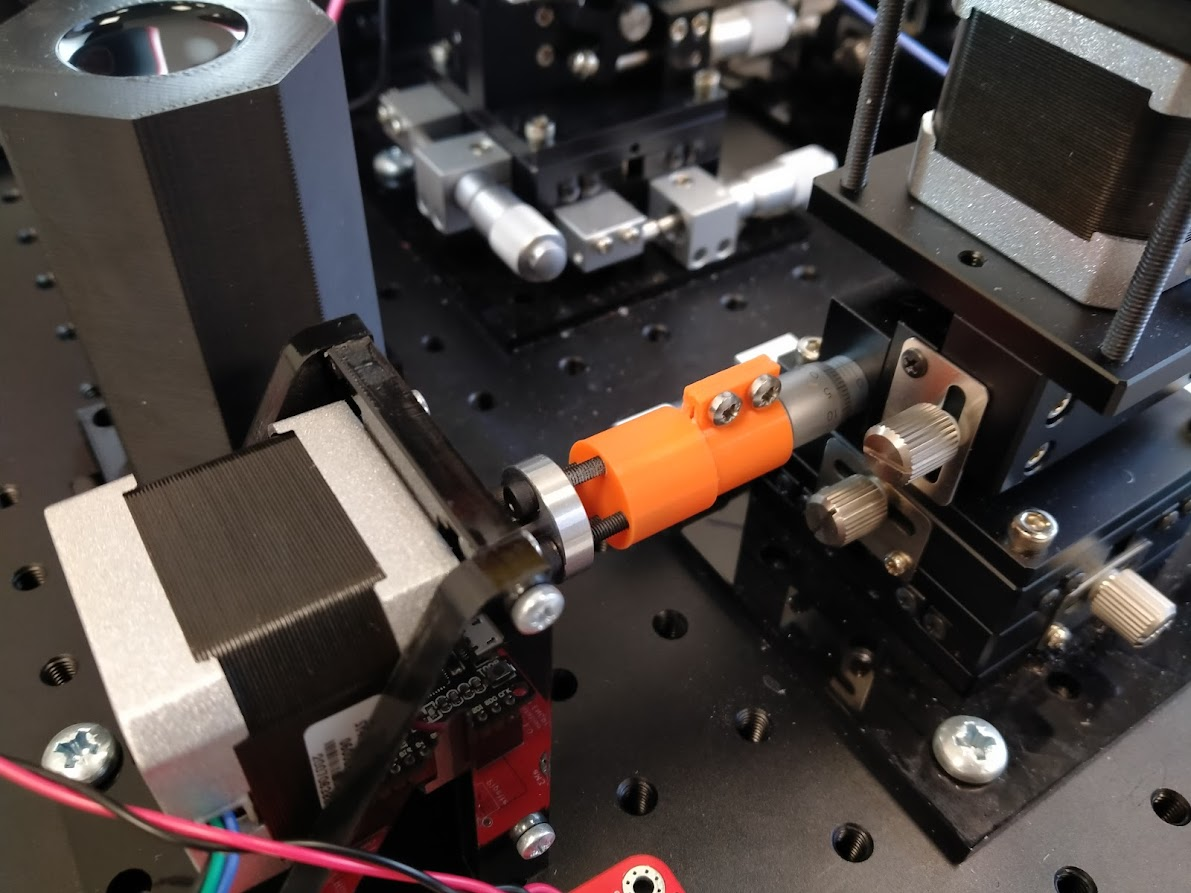
\includegraphics[width=0.4\textwidth]{img/impl_coup.jpg}
    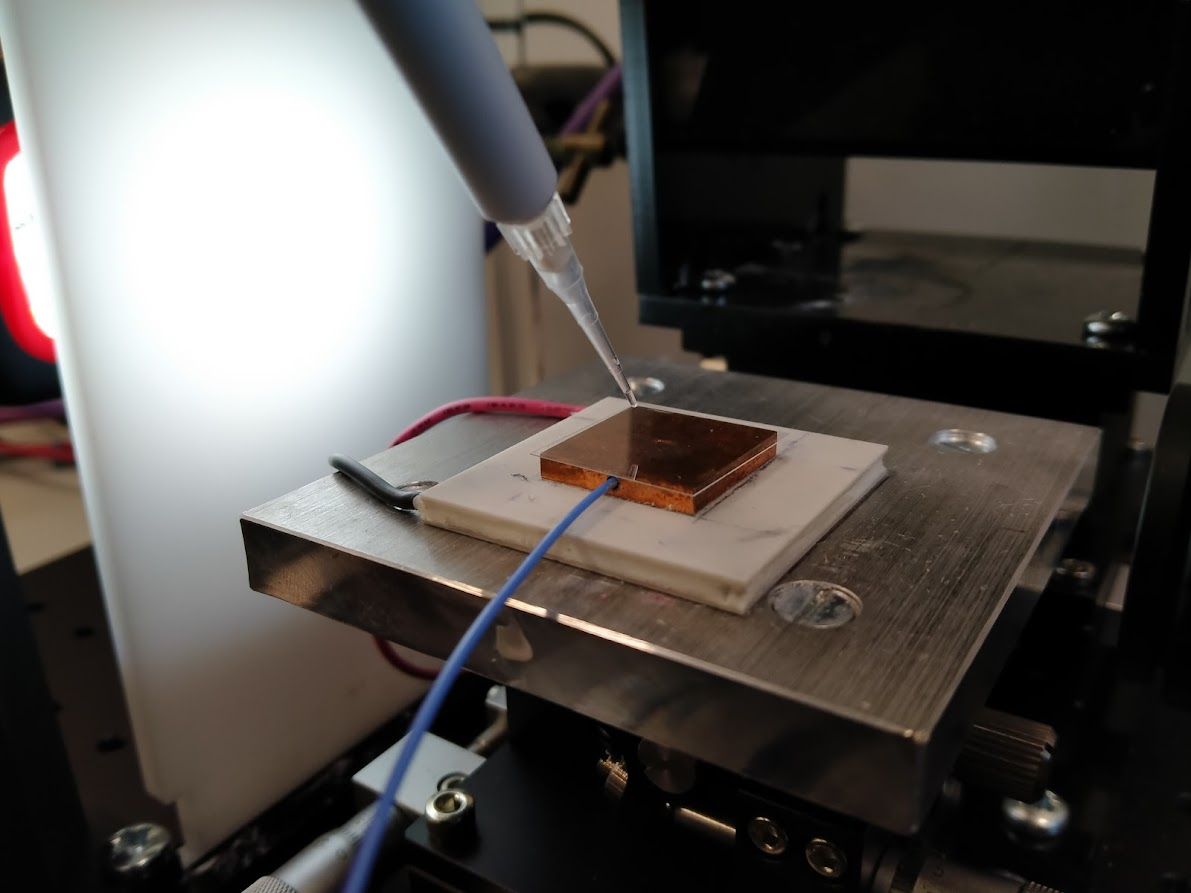
\includegraphics[width=0.4\textwidth]{img/new_stack.jpg}
\end{figure}

\section{Software}

//Insert Serial Command Table (maybe only appendix)

\subsection{Motorised Dispensing Controller}
ESP32 based system controller with serial interface for issuing commands. Provides functionality to:
\begin{itemize}
    \item Motorised stages, height and angular position
    \item e-Pipette droplet dispensing
\end{itemize}

\subsection{Environmental Monitor}

\begin{itemize}
    \item Auto sleeping, button wake upon
    \item Circuit-Python implementation
\end{itemize}

\subsection{LabView Temperature Logger}

\section{Electronic Design}

\begin{figure}
    \centering
    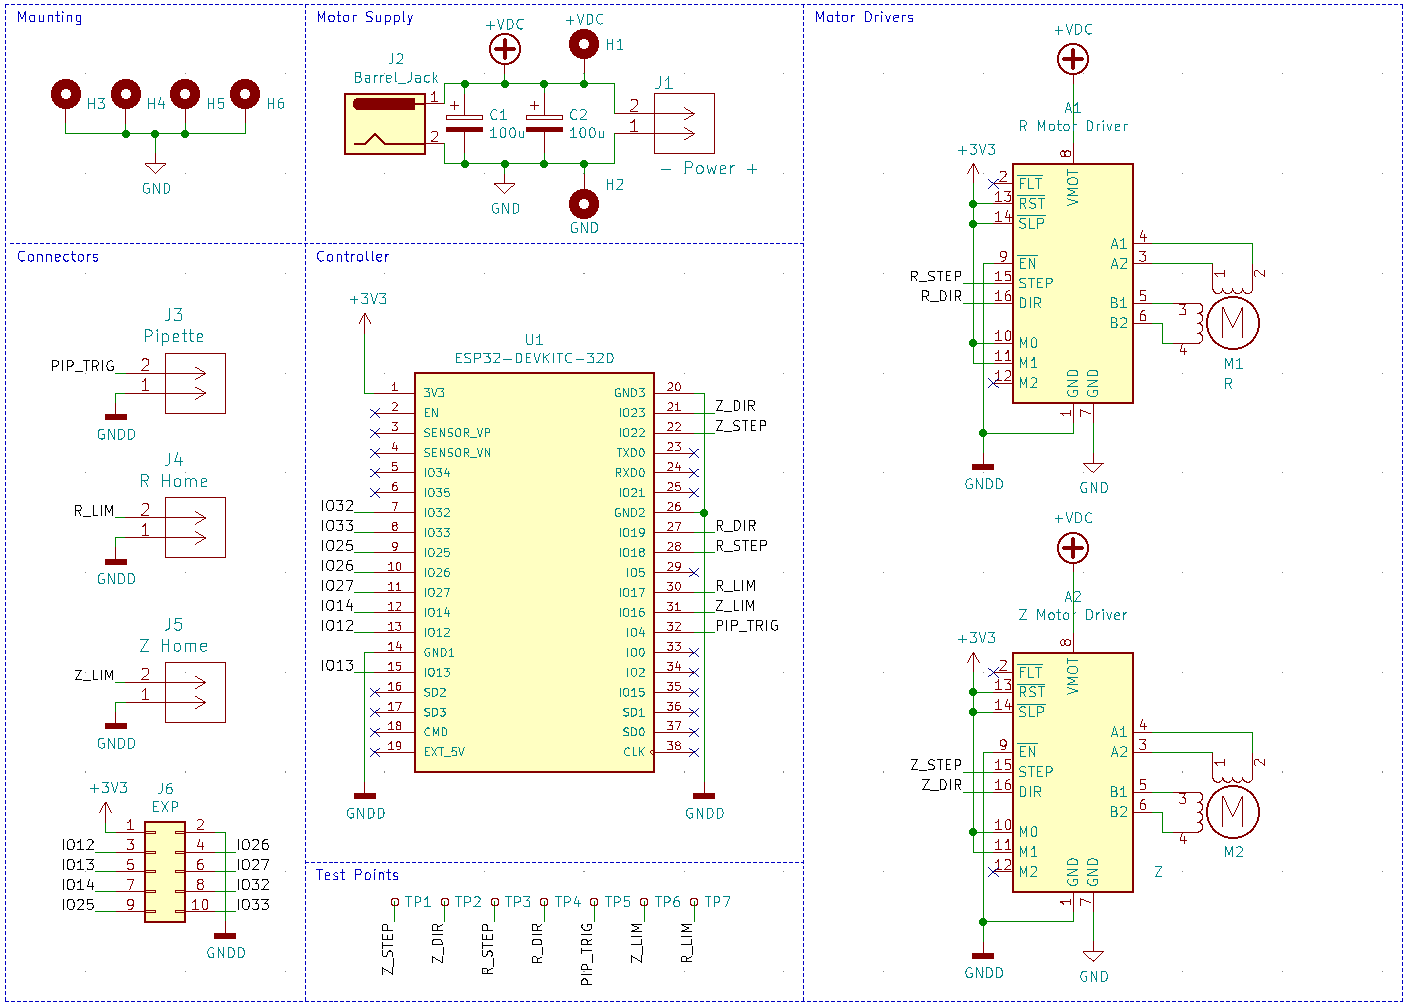
\includegraphics[width=0.4\textwidth]{img/schem.png}
    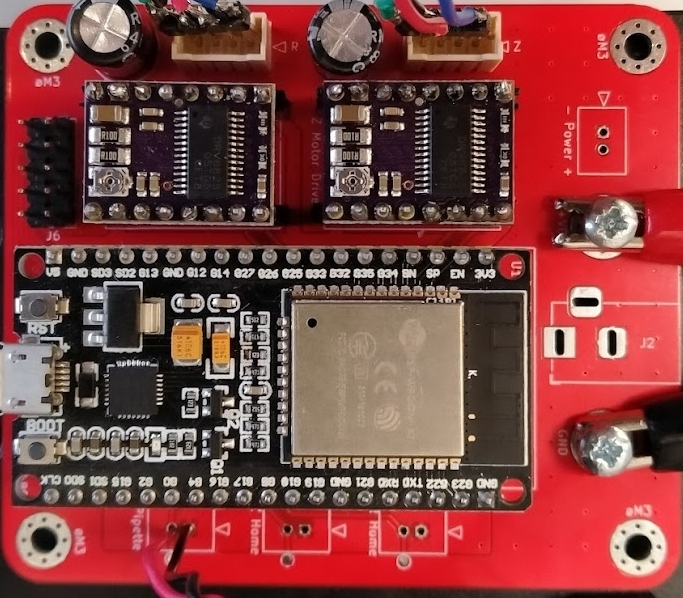
\includegraphics[width=0.4\textwidth]{img/control_pcb.jpg}
\end{figure}

\begin{itemize}
    \item full circuit
    \item pcb
    \item any and all adjustment found and made during implementation
\end{itemize}

\subsection{Motor Driving}

\subsection{Setup and Requirements}

\begin{itemize}
    \item characterised skipping issue at 100Hz, 180Hz-200hz in single step
    \item implemted micro stepping to solve
\end{itemize}

//TODO rewrite

Driving firmware was implemented on an ESP32 to validate its ability in producing the required pulse train step signal. The controller was required to produce N steps (pulses) at a set average speed, and ramp up and down that pulse speed at the head and tail of that signal.

Set values of 200 steps forward and back, at a speed of 200 steps per second, with max acceleration or 800 steps per second per second:

These pulses were captured on a second microcontroller listening for falling edges to trigger an interrupt routine to record and display that data.

\subsection{Results}

Figure \ref{fig:code}:a shows a successfully produced signal of 200 pulses with an inferred acceleration at its head/tail. This speed ramping is better illustrated in figure \ref{fig:code}:b showing the stepping change in pulses per second over the course of the pulse train.

\begin{figure}[h]
    \centering
    \begin{subfigure}{.45\textwidth}
        \centering
        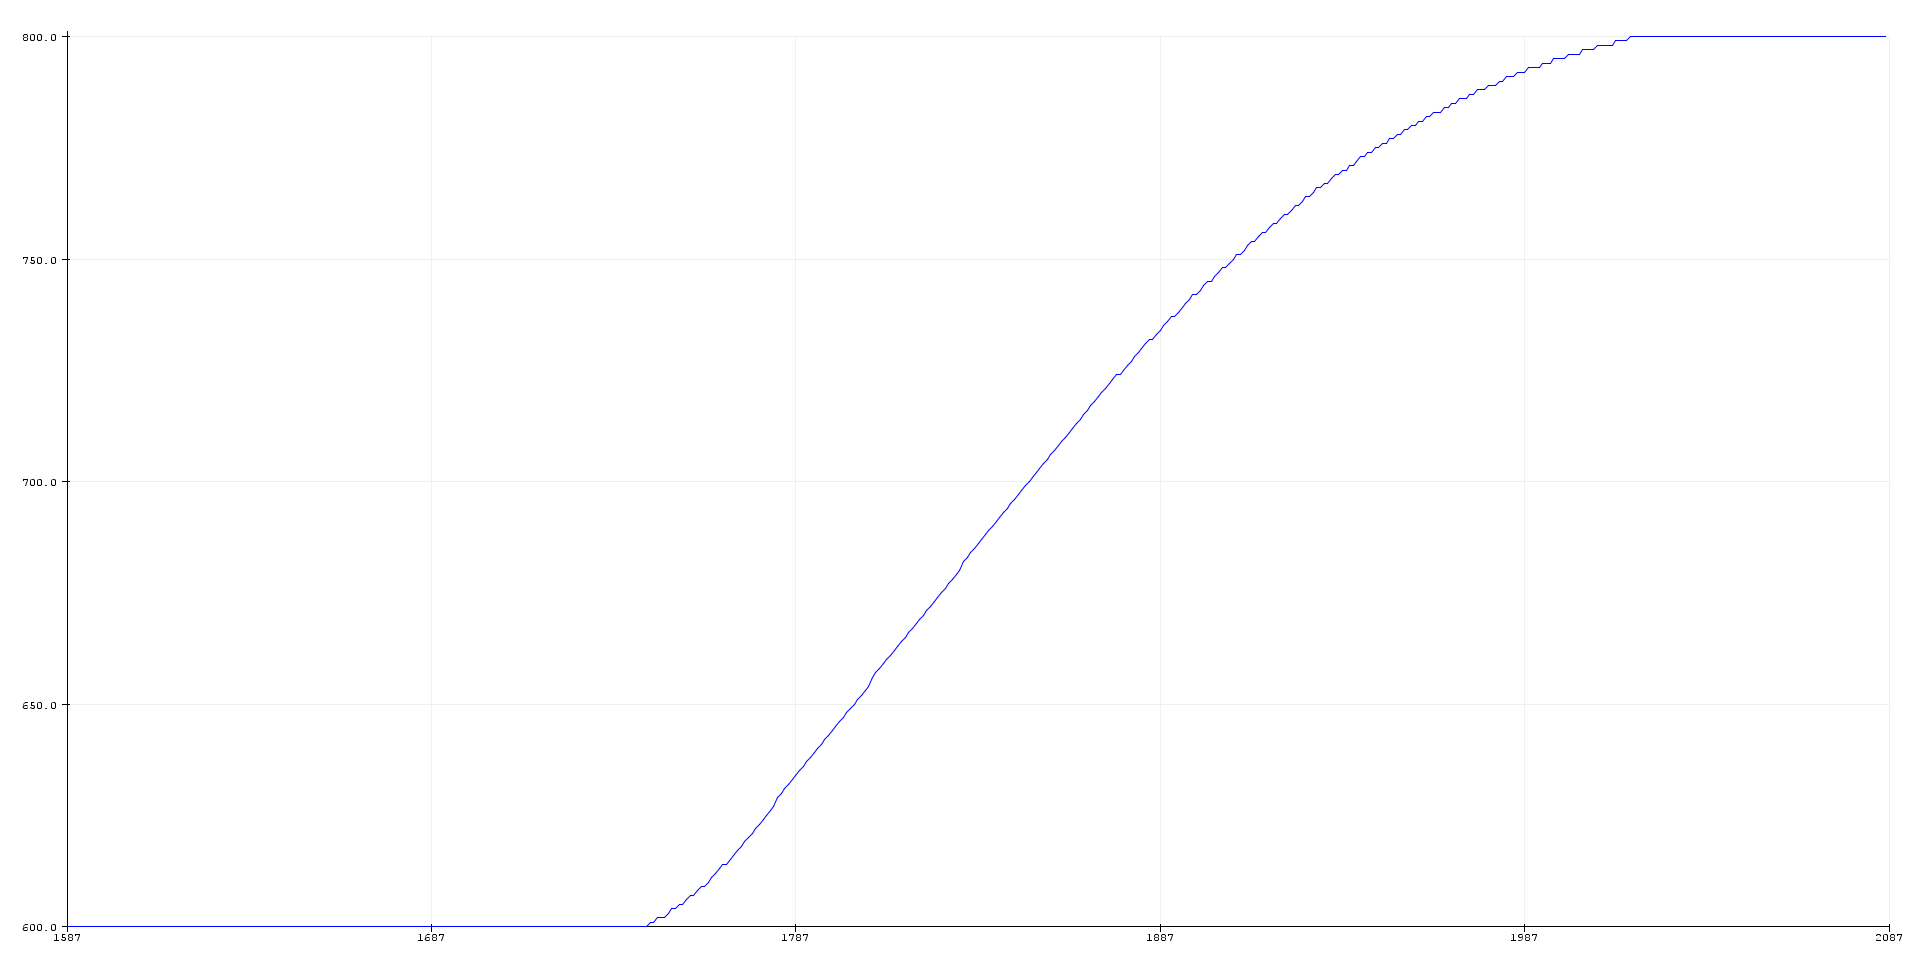
\includegraphics[width=0.8\linewidth]{img/stepper_pulses.PNG}
        \caption{Pulse Count}
    \end{subfigure}%
    \begin{subfigure}{.45\textwidth}
        \centering
        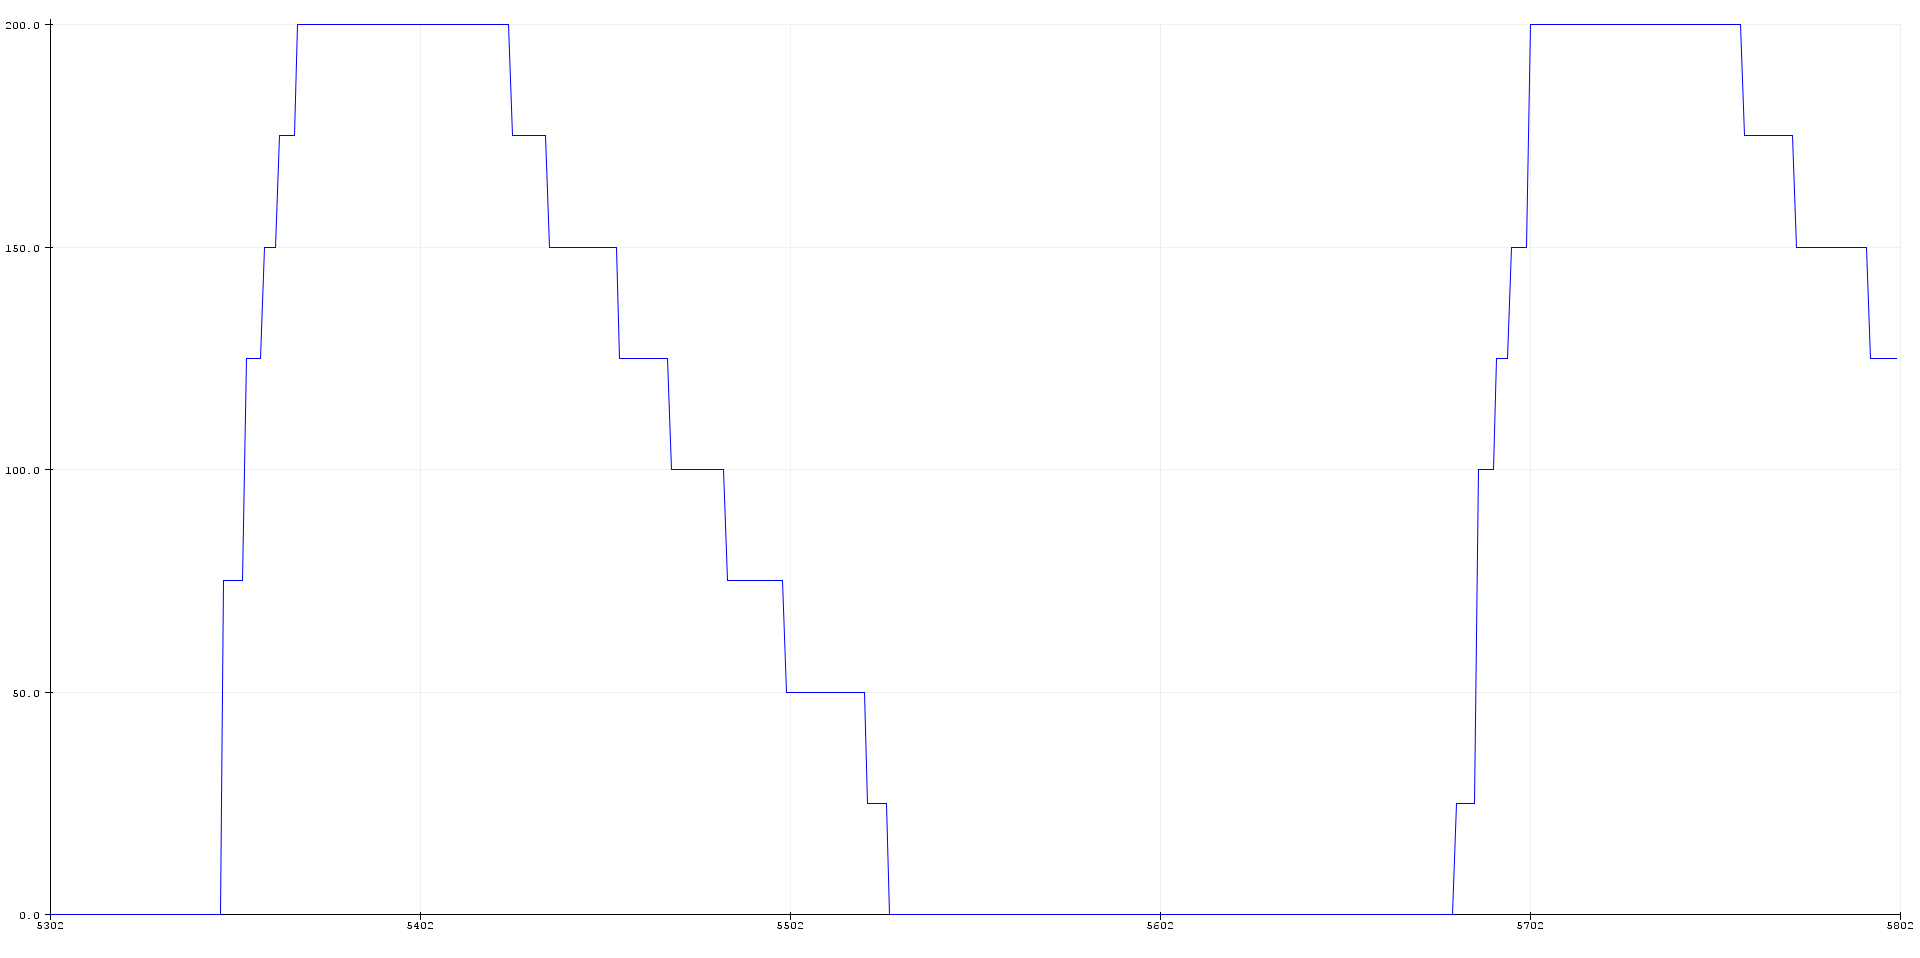
\includegraphics[width=0.8\linewidth]{img/stepper_pulse_acc.PNG}
        \caption{Pulses per Second}
    \end{subfigure}
    \caption{}
    \label{fig:code}
\end{figure}

\subsection{Pipette Triggering}
//TODO
\subsection{Environmental Monitoring}

\begin{figure}
    \centering
    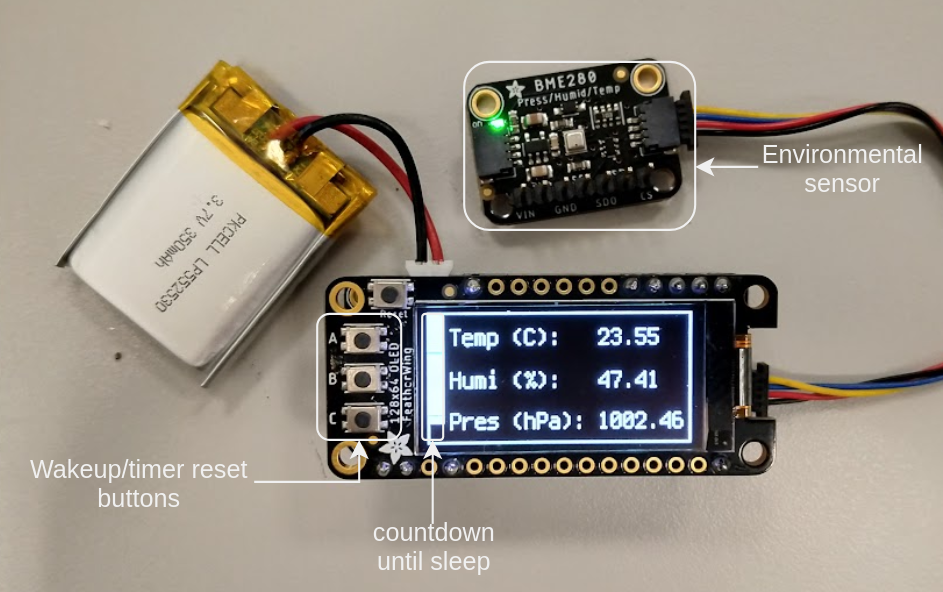
\includegraphics[width=0.4\textwidth]{img/env_mon.png}
\end{figure}